%\begin{figure}
%  \center
%  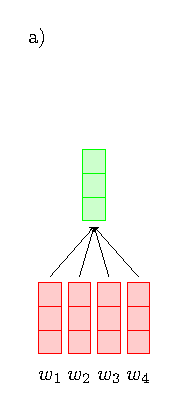
\includegraphics[scale=.7]{figures/avgsentencoder.pdf}
%  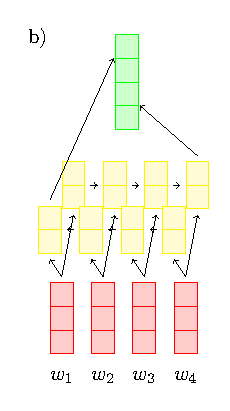
\includegraphics[scale=.7]{figures/rnnsentencoder.pdf}
%  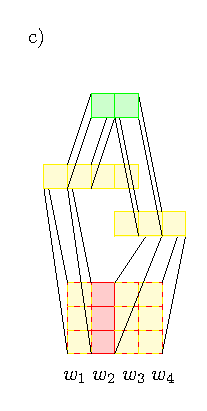
\includegraphics[scale=.7]{figures/cnnsentencoder.pdf}
%  \caption{Sentence encoder architectures: a) averaging encoder, b) RNN encoder
%           c) CNN encoder. Red indicates word embeddings, yellow indicates
%           RNN hidden states or convolutional activations, and green 
%           indicates the sentence embedding that is passed to the extractor
%           module.}
%    \label{fig:encoders}
%\end{figure}

%\hal{these descriptions are inconsistent in notation. in the first you use enc(s) but before you say h, and in other palces you say h below. h also switches between hidden state of the encoder and the output of the encoder. you'll also need to say somewhere that $w$ represents the word embedding of a word.}

%We treat each sentence $\sent = \wordEmb[1], \ldots, \wordEmb[\sentSize]$
%as a sequence of word embeddings, where 
%$\wordEmb[i] \in \mathcal{R}^\wordEmbSize$ are word embeddings and
%$\sentSize$ is the total number of words
%in the sentence. 
We experiment with three architectures for mapping sequences
of word embeddings to a fixed length vector: averaging, RNNs, and CNNs.
See Figure~\ref{fig:encoders} for a diagram of the three encoders.
Hyperparameter settings and implementation details can be found 
in the appendix.

\paragraph{Averaging Encoder} Under the averaging encoder, a sentence embedding
\sentEmb is simply the average of its word embeddings, i.e. $\sentEmb = \frac{1}{\sentSize} \sum_{i=1}^{\sentSize} \wordEmb[i]$.


%\hal{get rid of orphans.}
%
%$\operatorname{enc}(\sent) = \frac{1}{|\sent|} \sum_{\wemb \in \sent} \wemb$.
%\hal{probably better to write $\frac 1 {|s|} \sum_{i=1}^{|s|} w_i$ since set notation makes me wonder about words that appear more than once.}

\paragraph{RNN Encoder} When using  the \textit{RNN} sentence encoder,
a sentenc embedding is the 
concatenation 
of the
final output states of a forward and backward RNN over the sentence's word
embeddings. We use a Gated Recurrent Unit (GRU)  
for the RNN cell \cite{chung2014empirical}.
%since it has fewer parameters than the equivalent LSTM but with similar 
%performance . 
%Details in \autoref{app:rnnencoder}.

\begin{toappendix}
\section{Details on RNN Encoder} \label{app:rnnencoder}
  
Under the \textit{RNN} encoder, a sentence embedding is defined as
$\sentEmb = [\rSentEmb[\sentSize]; \lSentEmb[1]]$
where 
\begin{align} 
  \rSentEmb[0] = \mathbf{0} &;\quad 
       \rSentEmb[i] = \rgru(\wordEmb[i], \rSentEmb[i-1]) \\
  \lSentEmb[\sentSize + 1] = \mathbf{0} &;\quad 
       \lSentEmb[i] = \lgru(\wordEmb[i], \lSentEmb[i+1]),
%\lSentVec_i &= \lgru(w_i, \lSentVec_{i+1}) 
\end{align}
and $\rgru$ amd $\lgru$ indicate the 
forward and backward GRUs respectively, each with separate 
parameters.
\end{toappendix}

%\hal{
%  maybe you can make this more brief by saying sth like:
%  \begin{align}
%    \rSentVec_0 = \mathbf{0} &;\quad \rSentVec_{i+1} = \dots \\
%    \lSentVec_{|s|+1} = \mathbf{0} &;\quad \lSentVec_{i-1} = \dots
%  \end{align}
%  then you don't need to spe
%  }

\paragraph{CNN Encoder} The \textit{CNN} sentence encoder uses a series of 
convolutional feature maps to encode each sentence. This encoder is similar
to the convolutional architecture of \cite{kim2014convolutional} used for text
classification
tasks and performs a series of ``one-dimensional'' convolutions over 
word embeddings. The final sentence embedding $\sentEmb$ is a concatenation
of all the convolutional filter outputs after max pooling over time.

\begin{toappendix}
\section{Details on CNN Encoder} \label{app:cnnencoder}
The \textit{CNN} encoder has hyperparameters
associated with the window sizes $\maxWindowSize \subset \mathcal{N}$ of the convolutional filter 
(i.e. the number of words associated with each convolution) and the number of 
feature maps $\maxFeatureMaps$ associated with each filter
(i.e. the output dimension of each 
convolution). 
The \textit{CNN} sentence embedding $\sentEmb$ is computed as follows:
\begin{align}
 \specActivation_i &= \specConvBias 
    + \sum^\filterWindowSize_{j=1} \specConvWeight_j \cdot \wemb_{i + j -1}\\
  \specFeatureMap &= \max_{i\in 1,\dots, |\sent| - \filterWindowSize + 1} 
                      \relu\left(\specActivation_i\right) \\
 \sentEmb &= \left[\specFeatureMap | 
   \numFeatureMaps \in \{1, \ldots, \maxFeatureMaps\},
   \filterWindowSize \in \maxWindowSize
   \right]
\end{align}
where $\specConvBias\in\mathcal{R}$ and $\specConvWeight \in 
\mathcal{R}^{\filterWindowSize \times \wordEmbSize}$ are learned bias and filter
weight parameters respectively, and $\relu(x) = \max(0, x)$ is the rectified
linear unit activation.
\end{toappendix}


%%% Local Variables:
%%% mode: latex
%%% TeX-master: "dlextsum.emnlp18"
%%% End:
